% Results VI: prediction in the loop, the order-4 cap, shot-timed adversarial testing.
% Numbers: python/results/research/ (research_report.md, deconfound/, contact_order.md).
\textbf{Why this study.} A review of the frozen design raised two objections.
\begin{itemize}
\item \textbf{The prediction is cancelled trivially.} With deviation feedback the reference generator solves $(A_3+K)(\D)y_d=A_3(\D)\hat\theta+K(\D)\hat\theta$. On the estimator's polynomial nowcast this gives $(\D+20)^3(y_d-\hat\theta)=0$, whatever $A_3$ is. The Taylor polynomial agrees with $e^{st_p}$ only at $s=0$ in this loop (contact order 0), so the order-4 limit of Section~3.3 never binds.
\item \textbf{The homotopy idea was not implemented.} The hit probability used 17 hand-picked offsets, and the Monte Carlo drew random maneuvers instead of searching the directions that defeat the controller.
\end{itemize}
We therefore built every alternative behind a configuration flag, with the frozen design's defaults left untouched (bit-identical on all 1\,000 Monte Carlo seeds), and tested them on 1\,000 random and 1\,000 adversarial engagements each.

\subsection{Contact order: the order-4 cap, stated correctly}
\textbf{What we did.} We let the reference characteristic polynomial be $Q(x)=\sum_k q_kx^k$, $x=t_ps$, with $q_k=1/k!$ for $k\le m$, so $Q-e^x=O(x^{m+1})$ (\emph{contact order} $m$). We then added $f\le6$ free higher coefficients and maximised the least root damping $\zeta_{\min}$ by differential evolution.

\begin{figure}[H]
\centering
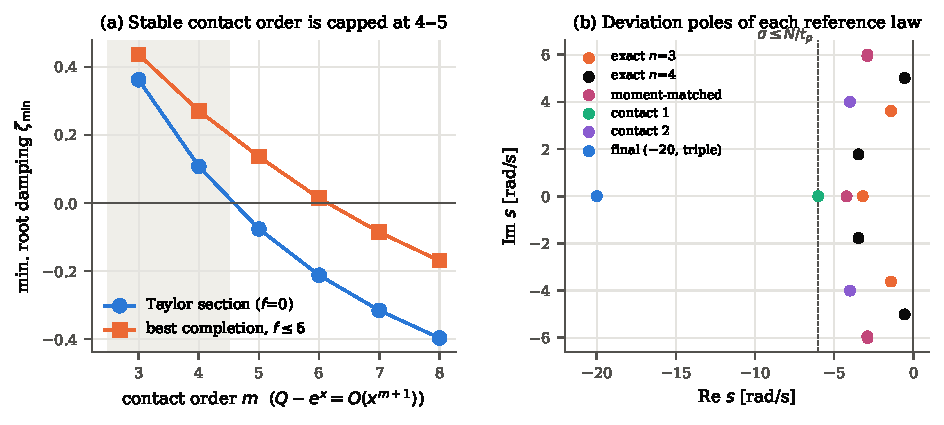
\includegraphics[width=\textwidth]{research_contact_order.pdf}
\caption{(a) Best least-root damping for each contact order. Pure Taylor sections (blue) are stable only up to order 4; extra free terms (orange) reach order 5 ($\zeta=0.136$) and order 6 only marginally ($\zeta=0.014$); no stable completion was found for orders 7--8. (b) Deviation poles of the reference laws tested. The dashed line is the decay bound $\sigma\le N/t_p=6$\,rad/s for a cubic that keeps the velocity prediction exact.}
\label{fig:contact}
\end{figure}

\obs{
\begin{itemize}
\item \textbf{The cap is real.} A stable loop can reproduce the $t_p$ shift to at most order 4--5 in $s$. Exact Taylor stops at $n=4$ with $\zeta=0.107$.
\item \textbf{Prediction in the loop is a choice of deviation poles.} In every mode the deviation obeys $P(\D)(y_d-\hat\theta)=0$, driven only by the estimator's correction at each radar update. Keeping first-order fidelity ($p_0=1$, $p_1=t_p$) forces $\sum 1/s_i=-t_p$, so the slowest pole decays at no more than $N/t_p$ (6\,rad/s for a cubic). The frozen design gives up that fidelity to place its poles at $-20$\,rad/s.
\item We tested six such laws: exact Taylor $n=3$ and $n=4$ ($T=1/A_n$); a moment-matched quintic $Q=A_3+0.741x^4/24+0.470x^5/120$, which keeps order-3 contact and whose two free coefficients maximise the slowest decay (2.9\,rad/s); contact order 1, $(1+s/6)^3$, which keeps only the velocity term and attains the bound; contact order 2, $((s^2+8s+32)/32)^2$; and blends of $A_3$ with the frozen design.
\item \textbf{Same large-signal handling for all.} Every law uses the frozen design's saturated acquisition cascade outside a hysteretic band and switches to its own linear law inside it ($|y_d-\hat\theta|<3$\,mrad and $|\dot y_d-\hat\theta'|<0.02$\,rad/s to enter, $>15$\,mrad to leave). No law is penalised by an unsaturated slew transient or by its initialisation.
\end{itemize}}
\takeaway{The order-4 limit binds on the \emph{transient} of the tracking loop, not on its steady state. It restricts which deviation poles may be chosen if the loop is to keep the Taylor prediction; it does not change what the turret tracks in steady state.}

\subsection{Shot-timed adversarial testing}
\textbf{What we did.} We work in the plane $(t,e)$, where $e$ is the target's signed cross-range offset from the beam. The obstacles are the firing events, the tubes $\{t_k\}\times[-\Reng,\Reng]$. A target path is a graph $e(t)$, so in this one-dimensional setting its class reduces to the sign of $e$ at each event, $h_k\in\{+1,0,-1\}$ (above, through = hit, below): the 1-D analogue of the homotopy classes of T-MPC \cite{degroot2024tmpc}, not a topological search in a richer space. The adversary \texttt{HG<seed>} takes a random base engagement and finds the frozen design's firing times. Before each event it reverses the normal acceleration at the envelope limit, with quintic ramps, toward the side that class \texttt{seed}\,\%\,5 requires (above, below, cross-down, cross-up, alternating). It chooses the lead time that maximises the frozen design's mean miss, and re-simulates once to check that the shots have not moved (a fixed-point step). The adversary is therefore white-box and non-causal: it knows the controller's shot times, which a real target cannot. All 1\,000 cases respect the envelope and the blackout rules.

\obs{
\begin{itemize}
\item \textbf{The classes steer the misses.} Where the frozen design misses, the side follows the attack: ``above'' seeds miss 38 above and 4 below, ``below'' seeds 1 above and 31 below.
\item \textbf{The adversary is weak.} Even with the shot times known, 633 of 1\,000 cases still had every pulse ``through'', and only 116 realised the intended class. All 1\,000 were intercepted.
\item The adversarial family is therefore worst-case evidence about \emph{where} misses come from. It is never pooled into the failure bound.
\end{itemize}}

\subsection{Results: nominal accuracy against adversarial robustness}
\begin{table}[H]
\centering\small
\caption{Reference laws on 1\,000 random (MC) and 1\,000 adversarial (HG) engagements, controller at 100\,Hz. Every configuration intercepted 1\,000/1\,000 in both families. ``Hits'' = pulses that hit. Exact $n=4$ uses an order-5 estimator ($\sigma=150$, $\tau=0.2$, not optimised).}
\label{tab:research}
\begin{tabular}{@{}lrrrrrr@{}}
\toprule
& \multicolumn{3}{c}{MC0--999} & \multicolumn{3}{c}{HG0--999}\\
\cmidrule(lr){2-4}\cmidrule(l){5-7}
Design & RMS [m] & misses & hits & RMS [m] & miss rate & hits\\
\midrule
\textbf{Frozen design} & \textbf{0.56} & \textbf{4} & \textbf{9193} & \textbf{1.21} & 2.67\% & \textbf{8901}\\
Blend $\alpha=0.2$ & 0.65 & 7 & 9187 & 1.41 & 3.57\% & 8697\\
Contact order 1 & 0.99 & 24 & 8907 & 1.90 & 1.08\% & 8515\\
Contact order 2 & 1.82 & 18 & 8443 & 3.09 & 1.08\% & 8116\\
Exact Taylor $n=3$ & 2.82 & 23 & 8033 & 3.83 & 0.94\% & 7802\\
Moment-matched & 2.94 & 33 & 7904 & 4.78 & 1.09\% & 7776\\
Exact Taylor $n=4$ & 4.91 & 23 & 7440 & 6.26 & 0.39\% & 7459\\
\bottomrule
\end{tabular}
\end{table}

\begin{figure}[H]
\centering
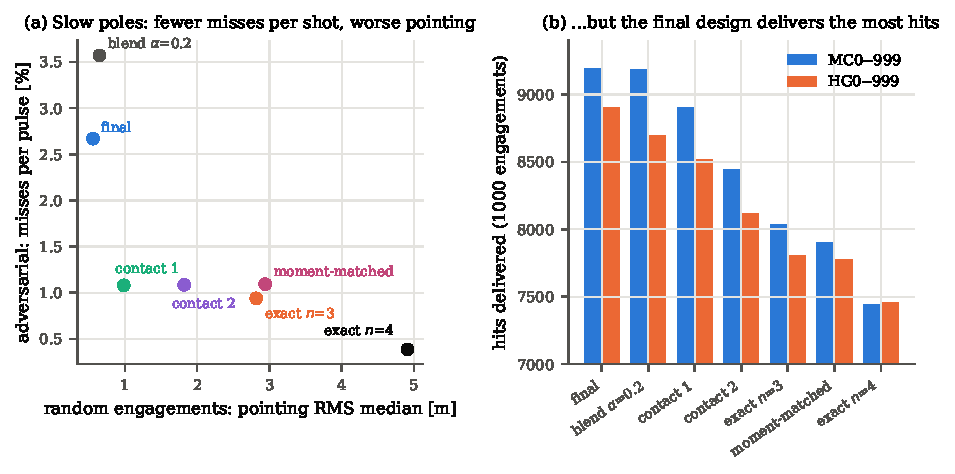
\includegraphics[width=\textwidth]{research_tradeoff.pdf}
\caption{(a) Nominal pointing error against the adversarial miss rate per pulse. (b) Hits delivered in each family. Slow deviation poles miss less often per shot, but they shoot less and hit less.}
\label{fig:tradeoff}
\end{figure}

\obs{
\begin{itemize}
\item \textbf{On random engagements the frozen design is best on every measure.} Every slower design has worse pointing (paired $p<10^{-160}$, Holm). The exact, moment-matched and contact-order laws also miss more (18--33 against 4, $p\le0.04$, Holm). The blends with $\alpha\ge0.1$ are not significantly different in misses.
\item \textbf{Under attack the per-pulse miss rate ranks the other way.} Slow poles miss 60--85\% fewer pulses per shot, because the 20\,rad/s loop chases each estimator correction and turns the lag the adversary induces into beam motion at the shot.
\item \textbf{But the frozen design still delivers the most hits.} The slow designs are on target 26--65\% of the time instead of 93\%, so the hit-probability gate holds their shots back. Time to first hit, which decides an interception, is within about 50\,ms for all designs.
\end{itemize}}

\subsection{Without the acquisition slew}
\textbf{What we did.} To check that the slow laws are not judged only on acquisition, we started the turret on the target's initial elevation (no slew) and re-ran seeds MC0--299 for the frozen design, exact Taylor $n=3$, contact order 1 and moment-matched.

\begin{table}[H]
\centering\small
\caption{No-slew start against the standard $0^\circ$ start, MC0--299 (pointing RMS median; misses / pulses).}
\label{tab:noslew}
\begin{tabular}{@{}lrrrr@{}}
\toprule
& \multicolumn{2}{c}{$0^\circ$ start} & \multicolumn{2}{c}{no slew}\\
\cmidrule(lr){2-3}\cmidrule(l){4-5}
Design & RMS [m] & misses & RMS [m] & misses\\
\midrule
\textbf{Frozen design} & \textbf{0.56} & 2 / 2752 & \textbf{0.52} & 1 / 3000\\
Contact order 1 & 0.98 & 5 / 2674 & 0.84 & 5 / 2781\\
Exact Taylor $n=3$ & 2.84 & 6 / 2415 & 1.31 & 7 / 2648\\
Moment-matched & 2.96 & 11 / 2384 & 1.69 & 7 / 2607\\
\bottomrule
\end{tabular}
\end{table}

\obs{
\begin{itemize}
\item Removing the slew halves the error of the exact and moment-matched laws, so part of their penalty is acquisition.
\item They still point 1.6--3.2 times worse than the frozen design, which barely changes. The remaining penalty is the slow deviation poles following the estimator's corrections, not initialisation or ringing from the slew.
\end{itemize}}

\subsection{Does the robustness survive an adversary tuned against each design?}
We re-ran the adversarial search against contact order 1 and exact Taylor $n=3$ on seeds 0--199, and played every adversary against every design (Fig.~\ref{fig:deconf}).

\begin{figure}[H]
\centering
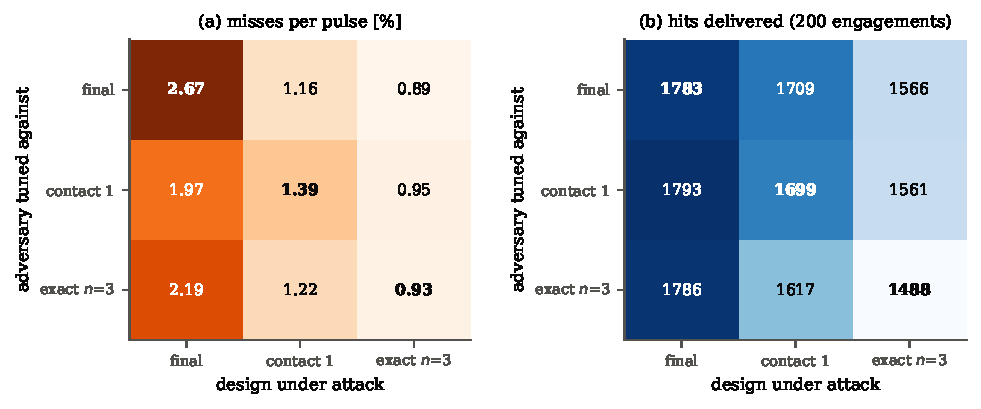
\includegraphics[width=\textwidth]{research_deconfound.pdf}
\caption{Attacker $\times$ defender on 200 engagements. Bold: each design against the adversary tuned on it. All 1\,800 engagements were intercepted.}
\label{fig:deconf}
\end{figure}

\obs{
\begin{itemize}
\item Each design is hit hardest by its own adversary (the diagonal). Its worst-case miss rate is 2.67\% for the frozen design, 1.39\% for contact order 1 and 0.93\% for exact Taylor $n=3$.
\item Exact Taylor $n=3$ beats the frozen design's miss rate under every adversary ($p\le0.008$). Contact order 1's advantage is not significant under its own adversary (36 vs 24 misses, $p=0.15$).
\item In hits delivered the frozen design wins every cell.
\end{itemize}}

\subsection{Homotopy fire planner and the remaining audit items}
\begin{itemize}
\item \textbf{Fire planner.} The planner uses 25 maneuver hypotheses scored by their sign pattern over the remaining recharge window, Gaussian spread from the noise-free covariance, and the plan-consistency rule of T-MPC \cite{degroot2024tmpc}. It hits 19\,ms earlier on random engagements but misses more there ($4\to11$) and fewer under attack ($244\to230$), neither significantly. It was not adopted; the mixture rule stays.
\item \textbf{Hit-probability calibration under attack.} On random engagements $\Phit$ at the pulses is calibrated (mean 99.91\% predicted, 99.96\% observed over 9\,197 pulses). Under the adversary it is overconfident: 99.74\% predicted against 97.33\% observed over 9\,145 pulses, and in the 0.95--0.99 bin 97.0\% against 64.1\% (117 pulses). The 17 maneuver classes hedge a constant acceleration since the last radar sample, not a reversal timed to the shot.
\item \textbf{Plant error.} With $R$, $L$, $J_{eq}$ and $b$ each drawn in $\pm20\%$ per engagement (controller nominal), the frozen design intercepted 1\,000/1\,000 with 6 misses in 9\,190 pulses and unchanged pointing (0.557\,m). These four parameters barely enter the feed-forward, whose dominant term $1001.5\,\dot y_d=(Rb+N^2K_tK_e)/(NK_t)\,\dot y_d\approx NK_e\,\dot y_d$ is set by the back-EMF constant. We therefore re-ran with all six parameters, $K_t$ and $K_e$ included (Table~\ref{tab:pert6}).

\begin{table}[H]
\centering\small
\caption{Six-parameter plant error ($R,L,J_{eq},b,K_t,K_e$ each $U(0.8,1.2)$), MC0--999, binned by the $K_e$ factor.}
\label{tab:pert6}
\begin{tabular}{@{}lrrr@{}}
\toprule
$K_e$ factor & runs & RMS median [m] & misses\\
\midrule
0.80--0.90 & 240 & 3.16 & 7\\
0.90--0.95 & 142 & 1.94 & 1\\
0.95--1.05 & 261 & 0.77 & 3\\
1.05--1.10 & 114 & 1.55 & 2\\
1.10--1.20 & 243 & 3.27 & 2\\
\midrule
all & 1\,000 & 1.69 & 15 / 8\,158\\
\bottomrule
\end{tabular}
\end{table}
All 1\,000 were intercepted and 99.82\% of pulses hit, but pointing RMS rose from 0.56 to 1.69\,m (paired $p<10^{-160}$), fewer pulses were fired (8\,158 against 9\,190) and the mean first hit was 0.18\,s later. The error correlates with $|\log K_e|$ (Spearman $\rho=0.71$) and hardly with $K_t$ ($\rho=0.04$), as the feed-forward predicts. The design is robust in interception but its accuracy depends on knowing $K_e$. Friction and backlash are not modelled and were not tested.
\item \textbf{Re-identification.} Removing it changed nothing measurable (MC 3 vs 4 misses, HG 245 vs 244).
\item \textbf{Envelope projection} activates in 44\% of random and 96\% of adversarial engagements (0.9 and 12 times per run), always on the acceleration estimate.
\end{itemize}

\takeaway{The order-4 cap and the shot-timed adversary are now real parts of the analysis, and both were tested. Neither overturns the frozen design, but the adversary exposes an overconfident $\Phit$ and the plant study a sensitivity to $K_e$. Keeping the Taylor prediction in the loop forces slow deviation poles, which cost far more pointing accuracy and hits than they save in per-shot misses under attack. The frozen design remains the submitted one.}
